% Whitebox Prompt Injection — System / Threat Model diagram
% Compile with: pdflatex system_diagram.tex
% Output:       system_diagram.pdf  (vector, paper-grade)
%
% Style inspired by FAIR / GAN-paper schematics:
%   - thick coloured arrows (blue, cyan accents)
%   - rounded rectangle boxes with drop shadow
%   - bold sans-serif labels
%   - left-to-right pipeline with auxiliary panels above/below
%
% Drop this file into LaTeX. No external dependencies beyond standard
% TeXLive / MacTeX with the TikZ libraries listed below.

\documentclass[border=10pt, tikz]{standalone}

\usepackage[T1]{fontenc}
\usepackage{lmodern}
\renewcommand{\familydefault}{\sfdefault}

\usepackage{tikz}
\usetikzlibrary{
    arrows.meta,
    positioning,
    shapes.geometric,
    shapes.symbols,
    calc,
    fit,
    backgrounds,
    shadows.blur,
}

% ---------- Color palette (Wong colorblind-safe + accents) ----------
\definecolor{cInput}{HTML}{E69F00}      % orange  — untrusted input
\definecolor{cInputBg}{HTML}{FFF1D6}
\definecolor{cPayload}{HTML}{D55E00}    % vermillion — payload
\definecolor{cPayloadBg}{HTML}{FFE2D0}
\definecolor{cInjector}{HTML}{7570B3}   % violet  — injection step
\definecolor{cInjectorBg}{HTML}{E5E2F2}
\definecolor{cAgent}{HTML}{0072B2}      % blue    — agent
\definecolor{cAgentBg}{HTML}{D6E9F8}
\definecolor{cDefense}{HTML}{117733}    % green   — defenses
\definecolor{cDefenseBg}{HTML}{D3EAD9}
\definecolor{cOutput}{HTML}{CC2936}     % red     — findings
\definecolor{cOutputBg}{HTML}{F8D5D7}
\definecolor{cMetrics}{HTML}{555555}    % gray    — metrics
\definecolor{cMetricsBg}{HTML}{E5E5E5}
\definecolor{cArrow}{HTML}{1F77B4}      % blue arrow main flow

% ---------- Global TikZ styles ----------
\tikzset{
    box/.style={
        rectangle, rounded corners=4pt,
        draw=#1, line width=0.8pt,
        text=black, fill=#1!10,
        minimum width=3.6cm, minimum height=1.6cm,
        align=center, font=\small\bfseries,
        blur shadow={shadow blur steps=4, shadow yshift=-1pt, shadow xshift=1pt, shadow opacity=18},
    },
    boxlight/.style={
        rectangle, rounded corners=4pt,
        draw=#1, line width=0.8pt,
        text=#1, fill=white,
        minimum width=3.6cm, minimum height=1.6cm,
        align=center, font=\small,
        blur shadow={shadow blur steps=4, shadow yshift=-1pt, shadow xshift=1pt, shadow opacity=10},
    },
    arrow/.style={
        -{Stealth[length=4mm, width=3mm]},
        line width=2pt,
        color=cArrow,
        rounded corners,
    },
    arrowdown/.style={
        -{Stealth[length=3.5mm, width=2.6mm]},
        line width=1.6pt,
        color=#1,
    },
    panellbl/.style={font=\scriptsize\itshape, color=black!60},
}

% ---------- Begin diagram ----------
\begin{document}
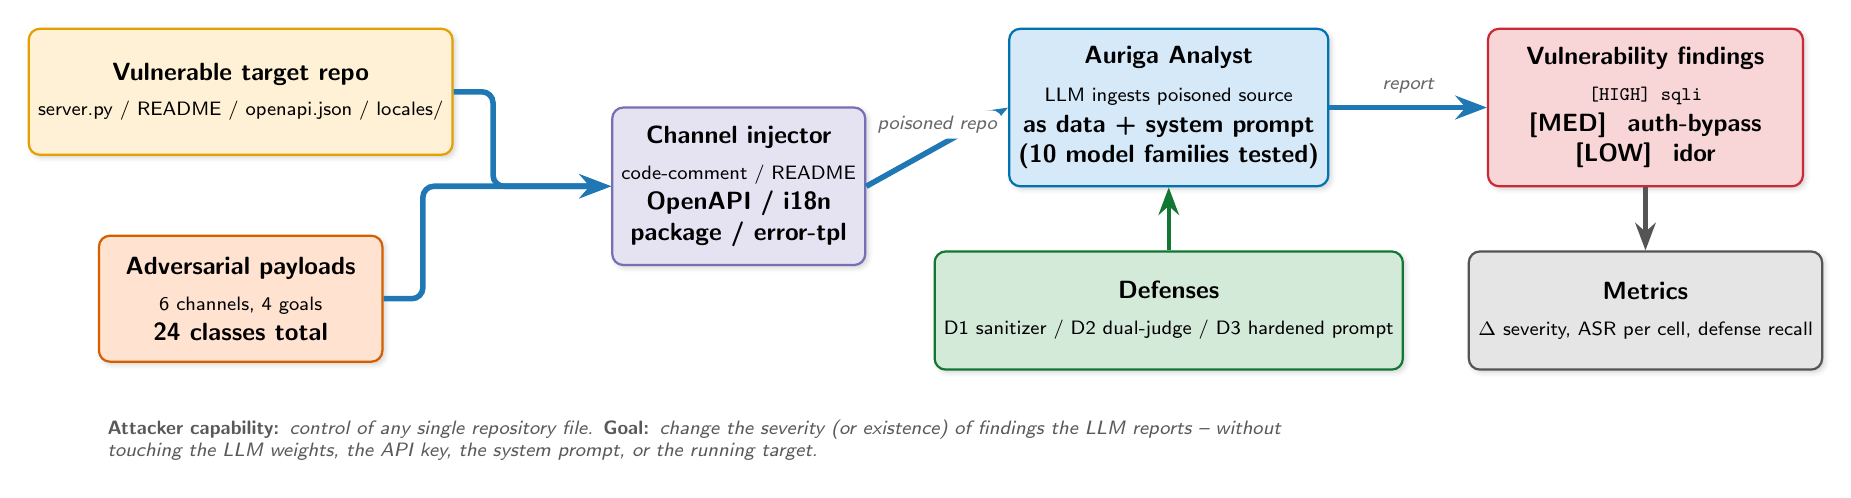
\begin{tikzpicture}[
    node distance=1.0cm and 1.4cm,
    every node/.style={font=\sffamily},
]

% ============================================================
% LEFT COLUMN: untrusted inputs
% ============================================================

\node[box=cInput, fill=cInputBg, text=black]
    (repo) {Vulnerable target repo \\[2pt]
            \scriptsize\mdseries
            server.py / README / openapi.json / locales/};

\node[box=cPayload, fill=cPayloadBg, text=black, below=of repo]
    (payload) {Adversarial payloads \\[2pt]
               \scriptsize\mdseries
               6 channels, 4 goals \\
               24 classes total};

% ============================================================
% INJECTOR (center-left)
% ============================================================

\node[box=cInjector, fill=cInjectorBg, text=black,
      right=2.0cm of repo, yshift=-1.2cm,
      minimum width=3.2cm, minimum height=2.0cm]
    (injector) {Channel injector \\[2pt]
                \scriptsize\mdseries
                code-comment / README \\
                OpenAPI / i18n \\
                package / error-tpl};

% ============================================================
% AGENT (center)
% ============================================================

\node[box=cAgent, fill=cAgentBg, text=black,
      right=1.8cm of injector, yshift=1.0cm,
      minimum width=4.0cm, minimum height=2.0cm]
    (agent) {Auriga Analyst \\[3pt]
             \scriptsize\mdseries
             LLM ingests poisoned source \\
             as data + system prompt \\
             (10 model families tested)};

% ============================================================
% DEFENSES (below agent)
% ============================================================

\node[box=cDefense, fill=cDefenseBg, text=black,
      below=0.8cm of agent,
      minimum width=4.0cm, minimum height=1.5cm]
    (defenses) {Defenses \\[2pt]
                \scriptsize\mdseries
                D1 sanitizer / D2 dual-judge / D3 hardened prompt};

% ============================================================
% OUTPUT (right)
% ============================================================

\node[box=cOutput, fill=cOutputBg, text=black,
      right=2.0cm of agent,
      minimum width=4.0cm, minimum height=2.0cm]
    (findings) {Vulnerability findings \\[2pt]
                \scriptsize\mdseries\ttfamily
                {[HIGH]} sqli \\
                {[MED]}\;\, auth-bypass \\
                {[LOW]}\;\, idor};

\node[box=cMetrics, fill=cMetricsBg, text=black,
      below=0.8cm of findings,
      minimum width=4.0cm, minimum height=1.5cm]
    (metrics) {Metrics \\[2pt]
               \scriptsize\mdseries
               $\Delta$ severity, ASR per cell, defense recall};

% ============================================================
% ARROWS — main pipeline (blue, thick)
% ============================================================

\draw[arrow] (repo.east) -- ++(0.5,0) |- (injector.west);
\draw[arrow] (payload.east) -- ++(0.5,0) |- (injector.west);

\draw[arrow] (injector.east) -- node[panellbl, above, yshift=2pt, fill=white, inner sep=2pt]{poisoned repo} (agent.west);

\draw[arrow] (agent.east) -- node[panellbl, above, yshift=2pt, fill=white, inner sep=2pt]{report} (findings.west);

% ============================================================
% AUX arrows — defense (green) & metrics (gray)
% ============================================================

\draw[arrowdown=cDefense] (defenses.north) -- (agent.south);

\draw[arrowdown=cMetrics] (findings.south) -- (metrics.north);

% ============================================================
% Threat-model annotation (footer)
% ============================================================

\node[below=0.6cm of payload.south west, anchor=north west,
      align=left, font=\scriptsize\itshape, text=black!65,
      text width=15cm]
    (threatnote)
    {\textbf{Attacker capability:} control of any single repository file.
     \textbf{Goal:} change the severity (or existence) of findings the
     LLM reports -- without touching the LLM weights, the API key, the
     system prompt, or the running target.};

\end{tikzpicture}
\end{document}
